\section{Vehicle description}

\subsection{The vehicle in general}

The vehicle is composed of two tracks enveloping 4 wheels, plus a gear connected to the differential gear box. The servomotor controls the steering of the vehicle by braking one track or another, so that the main motor only control the absolute speed and not the turning. The differential gear is powered directturningly by the motor.\\
A Hall sensor is plugged on each gear wheel to control the speed of each belt.\\
A platform of the same size of the vehicle \todo{have to put the dimensions and weight of the vehicle} is mounted on the vehicle, to support the PCB, the battery, and the sensors used to control the path of the vehicle.\\

The drive train is described on \figref{vehicleDescriptionDriveTrain}. This section describes more accurately each part of the vehicle.


\begin{figure}[H]
	\centering
	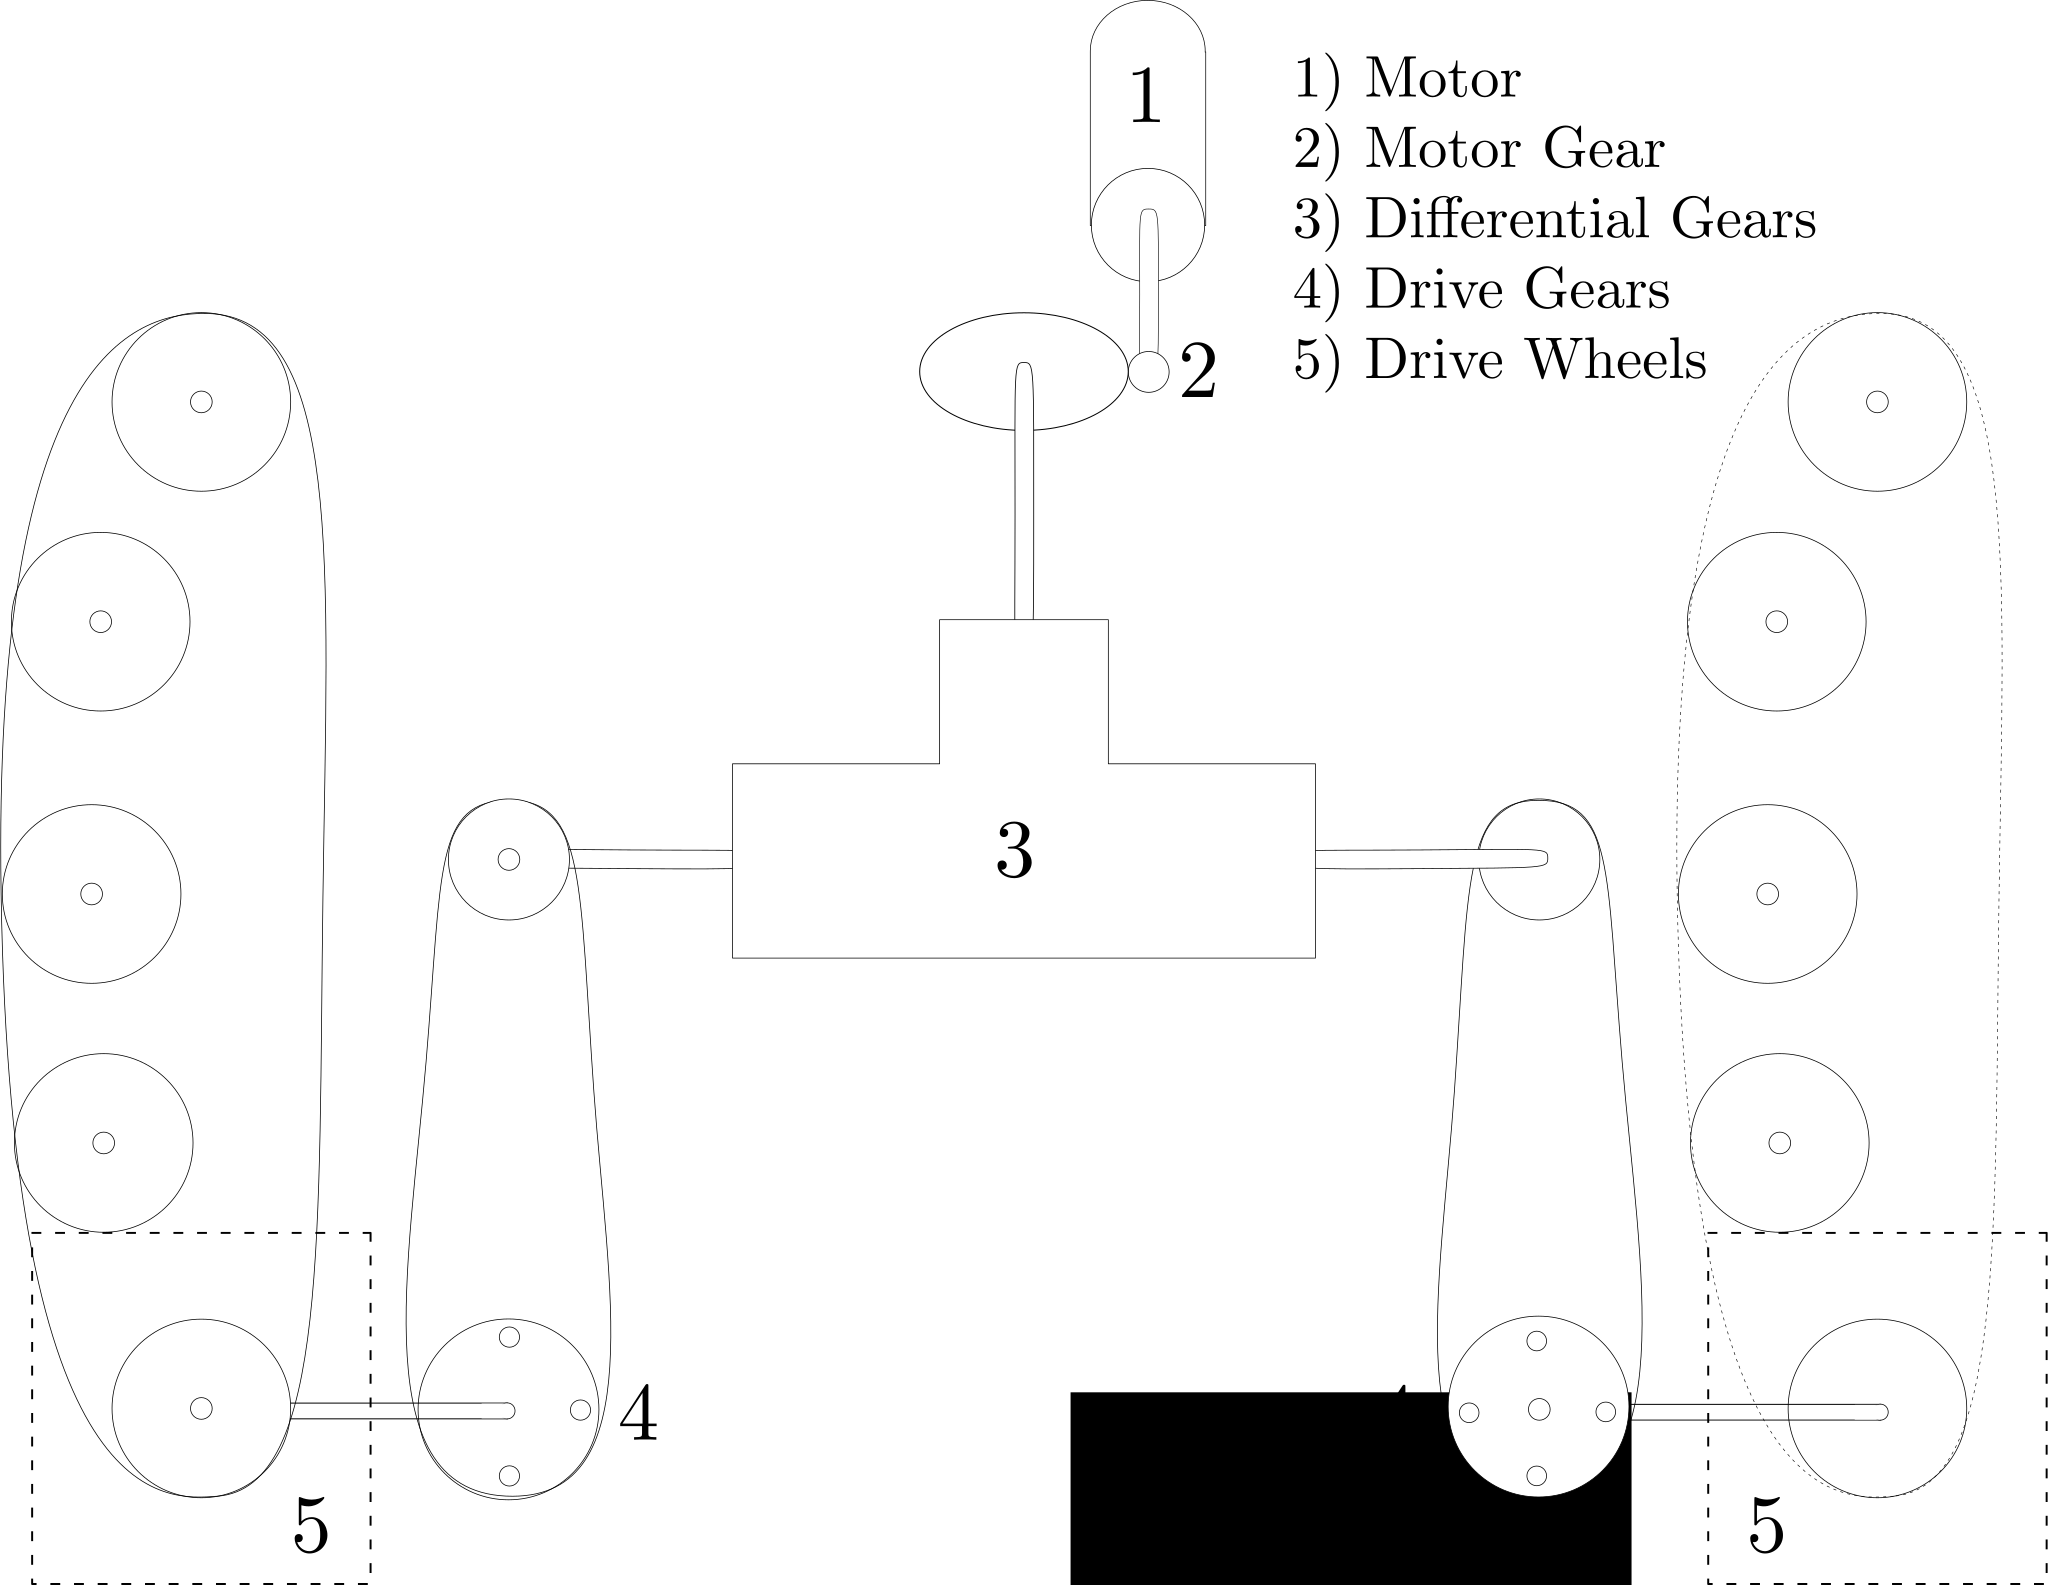
\includegraphics[scale=0.2]{figures/vehicleDescriptionDriveTrain.pdf}
	\caption{Illustration of the drive train of the vehicle.}
	\label{vehicleDescriptionDriveTrain}
\end{figure}